%This is the results section of my Master Thesis
\section{Results}\label{results}
In this section the results for the experiments explained in section \ref{experiments} will be showed. Different subjective test has been carried out for male and female voiced evaluating the two methods used for building the models (\ref{dpm}, \ref{adapt}).\\
\subsection{Training and Test Data}\label{ttd}
For the different methods and genres the amount of data have been different.
\subsubsection{Male voice}
For the different techniques the amount of data for the male voice is:
\begin{itemize}
	\item Dependent model (section \ref{dpm}): the same amount of data has been used for each emotion. The total amount of data per emotion is 489 sentences (around one hour of recording speech)
	\item Adaptation model (section \ref{adapt}): in this case the amount of data used for the training is all the data of the dependent models, which is 2445 sentences, and then all the data for each model to perform the adaptation.
\end{itemize}
Before synthesizing the test labels one of the models created has to be chosen as the better, for that reason a validation test has been done with 15 sentences of other speaker. Once the model has been chosen twenty sentences from the Albayzin contest have been used for the subjective test.
\subsubsection{Female voice}
For the different techniques the amount of data for the female voice is:
\begin{itemize}
	\item Dependent model (section \ref{dpm}): with the female voice the amount of data is not the same for each emotion, for the neutral emotion less sentences (504) are used than with the other emotions (around 605 sentences) .
	\item Adaptation model (section \ref{adapt}]): for the female voice, as it has less quality and with the average model a more robust model is wanted, a lot of data is used:  all the data of the dependent models (2922 sentences) plus the data of other 8 speakers (2808 sentences) , which makes a total of 5730 sentences. 
\end{itemize}
For the female voice no so many models has been created due to that in the adaptation the amount of data is too big and it takes more than a week to perform one training. In the dependent models the same models than in the male voice were obtained but the realignment didn't have good results in this case.The validation and test sentences are the same as for the male voice. All this information is compacted in table \ref{nutt}.\\
\begin{table}[!htb]
\begin{changemargin}{-2.6cm}{-4cm}
\begin{tabular}{|c|c|c|c|c|c|c|c|c|}
\hline 
\backslashbox{\textbf{Voice}}{\textbf{\#sent}} & \textbf{anger} & \textbf{happiness} & \textbf{neutral} & \textbf{sadness} & \textbf{surprise} & \textbf{average} & \textbf{validation} & \textbf{test} \\ 
\hline 
\textbf{Male} & 489 & 489 & 489 & 489 & 489 & 2445 & 15 & 20 \\ 
\hline 
\textbf{Female} & 605 & 603 & 504 & 605 & 605 & 5730 & 15 & 20 \\ 
\hline 
\end{tabular}  
\end{changemargin}
\caption{\label{nutt}Number of utterances used in train, validation and test}
\end{table}
\subsection{Test}\label{test}
As the purpose of the test is to compare GlottHMM with STRAIGHT the test has been divided into two parts.\\
In the first one the quality and the naturalness of the vocoder is tested, so two audio files are showed (A and B) and the next questions are asked in the test:
\begin{itemize}
	\item Choose the file that represent better the emotion (A or B)
	\item Choose the file that is more natural (A or B)
	\item Choose for both files the level of emotion (from poor to very high)
	\item Choose for both files the level of naturalness (from poor to very high)
\end{itemize}
In the second one the test is focused on the speaker voice, so it is asked to choose the file (A or B) with the voice more similar to the original speaker.\\
In the test the listeners are not going to listen to all the audio files, so the files showed in the test have been randomized using Latin square (\ref{anexo}), so that way nobody has control over the test.\\
In order to obtain enough results, three test have been performed. One for each dependent model and other one for the adaptation models. The reason for doing the adaptation test together was the difficulty to find listeners for the test.\\
\subsection{Male Voices Results}\label{maleres}
Here the results for the male voices and the two different methods will be showed.\\
\subsubsection{Dependent Model Results}\label{mdpmresults}
The results for the dependent model for the male voice are showed in figures \ref{joa1-ES-1}, \ref{joa1-MOS-1}, \ref{joa2-ES-1} and \ref{joa2-MOS-1}. Puede que haga 2 si las mezclo pero una al lado de la otra no creo que quepan y como son distintas no tiene sentido puedo agruparlas ES y MOS...
\begin{figure}[!htb]
	\begin{center}
	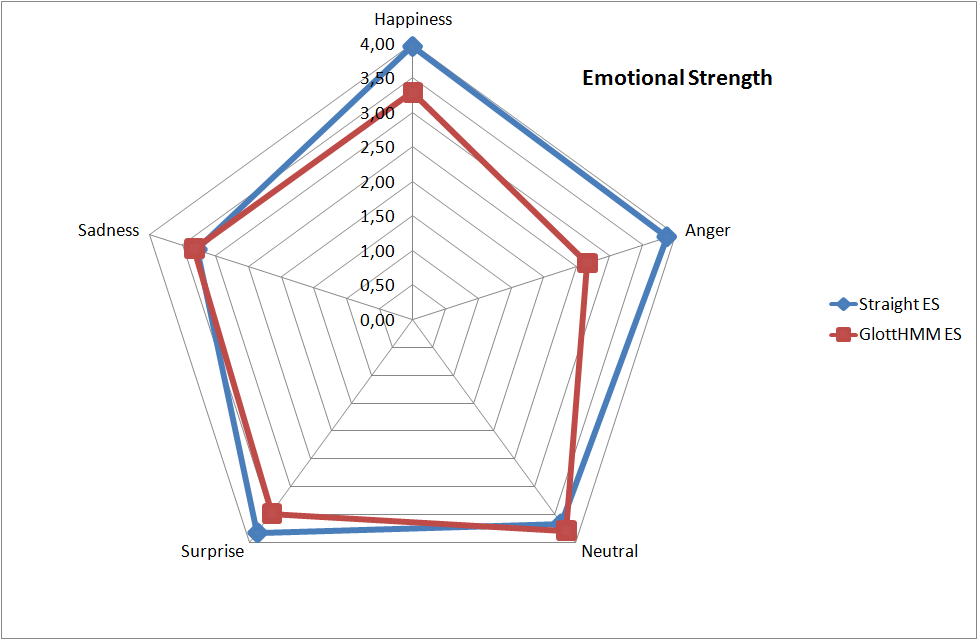
\includegraphics[width=1\textwidth]{results/Vocoders1_joa_ES.png}
	\end{center}
	\caption{\label{joa1-ES-1}ES representation for the emotional strength}
\end{figure}
\begin{figure}[!htb]
	\begin{center}
	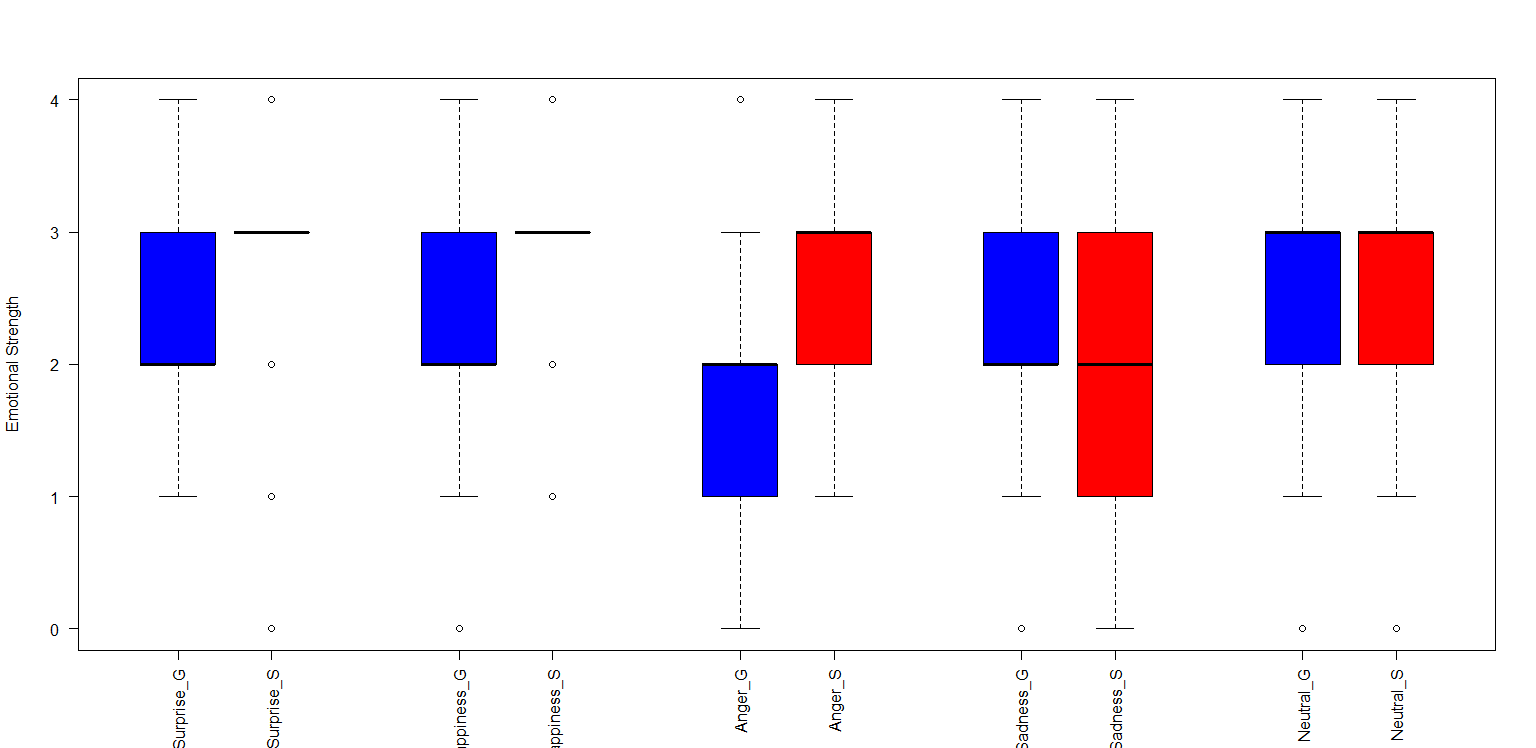
\includegraphics[width=1\textwidth]{results/Vocoders1_joa_ES_boxplot.png}
	\end{center}
	\caption{\label{joa1-MOS-1}ES boxplot representation for the emotional strength}
\end{figure}
\begin{figure}[!htb]
	\begin{center}
	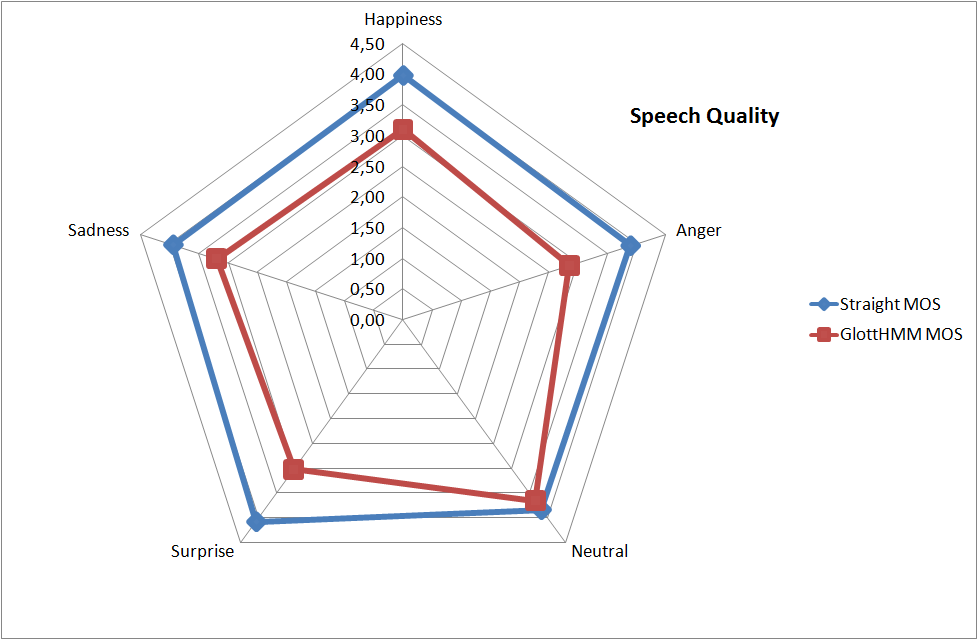
\includegraphics[width=1\textwidth]{results/Vocoders1_joa_MOS.png}
	\end{center}
	\caption{\label{joa2-ES-1}MOS representation for the speech quality}
\end{figure}
\begin{figure}[!htb]
	\begin{center}
	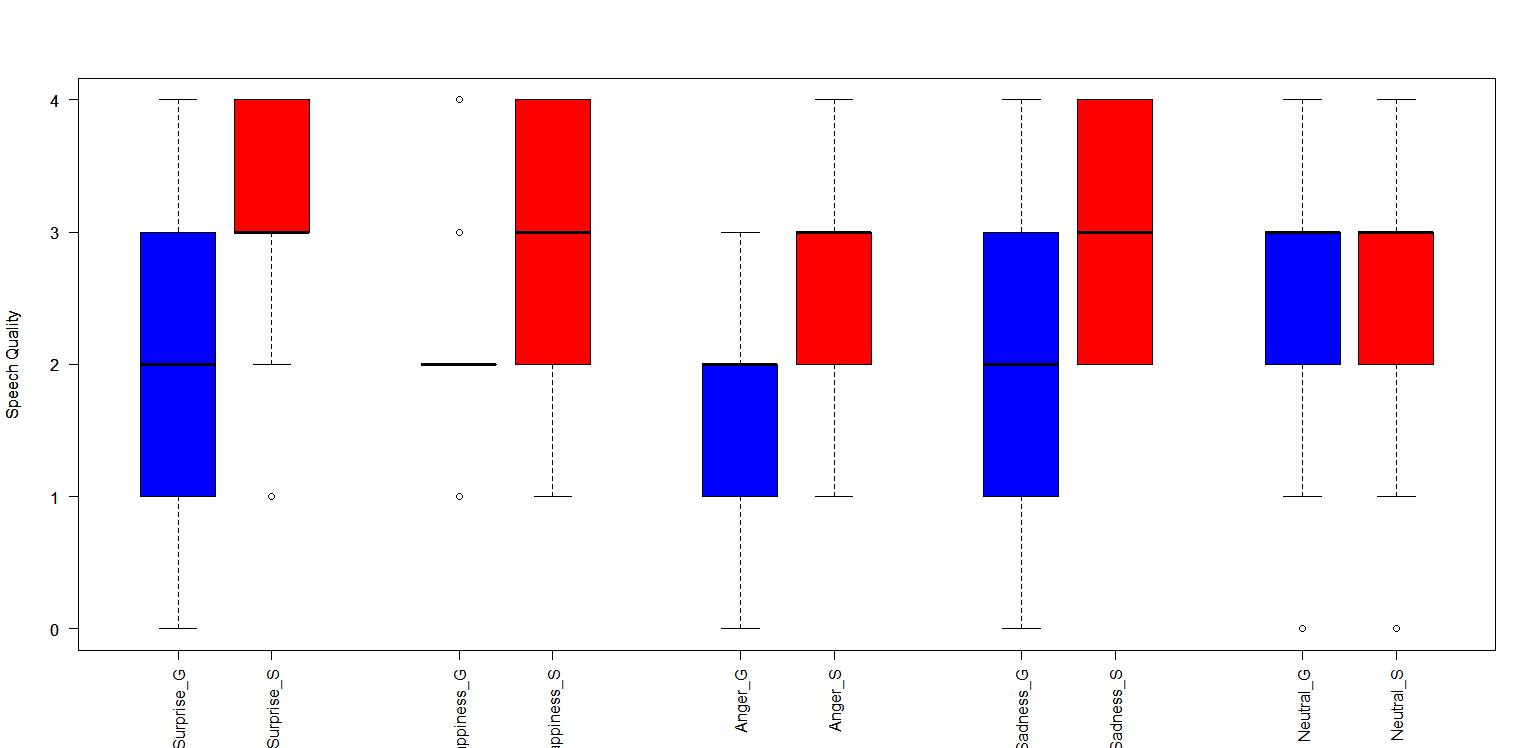
\includegraphics[width=1\textwidth]{results/Vocoders1_joa_MOS_boxplot.png}
	\end{center}
	\caption{\label{joa2-MOS-1}MOS boxplot representation for the speech quality}
\end{figure}

Faltan resultados del parecido de la voz al original, si estan pero en formato tabla en la parte SIM  y MOS es Mean Opinion Score

\subsubsection{Adaptation Model Results}\label{madaptresults}
\subsection{Female Voices Results}\label{femaleres}
Here the results for the female voices and the two different methods will be showed.\\
\subsubsection{Dependent Model Results}\label{fdpmresults}
\subsubsection{Adaptation Model Results}\label{fadaptresults}